The largest absolute error in any single timestep of our simulation is given by
\begin{equation}
  \Delta_{\text{max}, k} = \max_i |\bold{r}_{i,\text{exact}} - \bold{r}_i|
\end{equation}

We estimate the convergence rate by evaluating the change in maximum absolute error
relative to the change in step size. We write this as
\begin{equation}
  r_{\text{err}} = \frac{1}{3}\sum_{k=2}^4\frac{\log(\Delta_{\text{max}, k}) - \log(\Delta_{\text{max}, k-1})}{\log{(h_k)} - \log(h_{k-1})}
\end{equation}

\begin{figure}
  \centering
  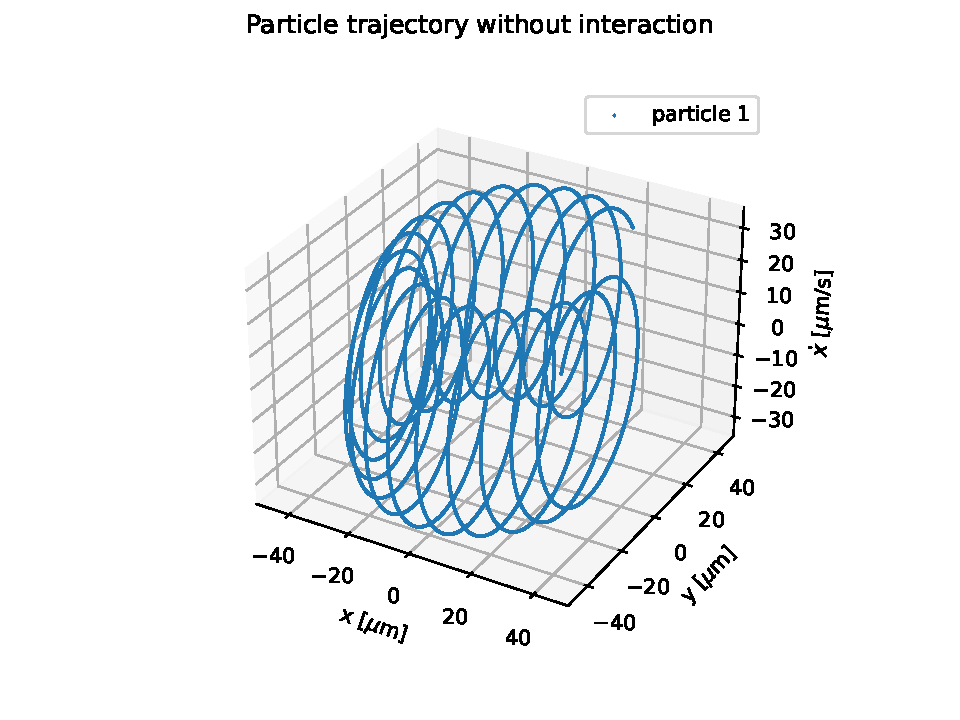
\includegraphics[scale = 0.7]{../figures/3d_phase.pdf}
  \caption{The phase space trajectory of a particle with no interactions. It seems
    to encircle a torus.}
\label{fig:torus}
\end{figure}


The proposed torus is mentioned in the \autoref{results}. We have not stored data from a simulation
that would verify that the trajectory closes in on itself after encircling the trap's centre.
